%%%%%%%%%%%%%%%%%%%%%%%%%%%%%%%%%%%%%%%%%
% fphw Assignment
% LaTeX Template
% Version 1.0 (27/04/2019)
%
% This template originates from:
% https://www.LaTeXTemplates.com
%
% Authors:
% Class by Felipe Portales-Oliva (f.portales.oliva@gmail.com) with template 
% content and modifications by Vel (vel@LaTeXTemplates.com)
%
% Template (this file) License:
% CC BY-NC-SA 3.0 (http://creativecommons.org/licenses/by-nc-sa/3.0/)
%
%%%%%%%%%%%%%%%%%%%%%%%%%%%%%%%%%%%%%%%%%

%----------------------------------------------------------------------------------------
%	PACKAGES AND OTHER DOCUMENT CONFIGURATIONS
%----------------------------------------------------------------------------------------

\documentclass[
	12pt, % Default font size, values between 10pt-12pt are allowed
	%letterpaper, % Uncomment for US letter paper size
	%spanish, % Uncomment for Spanish
]{../Template/fphw}

% Template-specific packages
\usepackage[utf8]{inputenc} % Required for inputting international characters
\usepackage[T1]{fontenc} % Output font encoding for international characters
\usepackage{mathpazo} % Use the Palatino font

\usepackage{graphicx} % Required for including images

\usepackage{booktabs} % Required for better horizontal rules in tables

\usepackage{listings} % Required for insertion of code

\usepackage{enumerate} % To modify the enumerate environment


% Additional packages needed
\usepackage{amsmath}
\usepackage{enumitem}
\usepackage{mwe}

%----------------------------------------------------------------------------------------
%	ASSIGNMENT INFORMATION
%----------------------------------------------------------------------------------------

\title{Homework \#1} % Assignment title

\author{Mao Nishino} % Student name

\date{February 13th, 2024} % Due date

\institute{Florida State University \\ Department of Computer Science} % Institute or school name

\class{Deep and Reinforcement Learning Fundamentals (CAP5619-0001.sp24)} % Course or class name

\professor{Dr. Xiuwen Liu} % Professor or teacher in charge of the assignment

%----------------------------------------------------------------------------------------

\begin{document}

\maketitle % Output the assignment title, created automatically using the information in the custom commands above

%----------------------------------------------------------------------------------------
%	ASSIGNMENT CONTENT
%----------------------------------------------------------------------------------------

\section*{Question 1}

\begin{problem}
	As neural networks are typically trained using (stochastic) gradient descent optimization
algorithms, properties of the activation functions affect the learning. Here we divide the domain of an activation
function into: 1) fast learning region if the magnitude of the gradient is larger than 0.99, 2) active learning region if
the magnitude of the gradient is between 0.01 and 0.99 (inclusive), 3) slow learning region if the magnitude of the
gradient is larger than 0 but smaller than 0.01, and 4) inactive learning region if the magnitude of the gradient is 0.
For each of the following activation functions, \textbf{plot} its gradient in the range from -5 to 5 of the input and then \textbf{list}
the four types of regions. If the gradient is not well defined for an input value, indicate so and then use any reasonable
value.

\begin{enumerate}[label = (\arabic*)]
    \item Rectified linear unit \( f(z) = \begin{cases} z & \text{if } z \geq 0 \\ 0 & \text{otherwise} \end{cases} \)
    \item Logistic sigmoid activation function \( f(z) = \sigma(z) = \frac{1}{1+e^{-z}} \) 
    \item Piece-wise linear unit \( f(z) = \begin{cases} 0.1z+0.9 & \text{if } z> 1 \\ z & \text{if }1\geq z\geq -1 \\ 0.1z-0.9 & \text{Otherwise} \end{cases} \) 
    \item Swish \(f(z) =  z\sigma(2.5z)\), where $\sigma(z) = \frac{1}{1+e^{-z}}$.
    \item Exponential Linear Unit (ELU) \( f(z) = \begin{cases} z & \text{if } z \geq 0 \\ 0.05(e^z-1) & \text{otherwise} \end{cases} \) (Note here is a special case of the general ELU function with $\alpha=0.05$.)
\end{enumerate}

\end{problem}

%------------------------------------------------

\subsection*{Answer}
We will first find the gradients analytically and then show the plot and the list(See Figure \ref{fig:gradients_q1}).

\begin{enumerate}[label = (\arabic*)]
\item The gradient of the ReLU function is \( f'(z) = \begin{cases} 1 & \text{if } z > 0 \\ \text{undefined} & z=0\\ 0 & z<0 \end{cases}\). In Figure \ref{fig:gradients_q1}, the value of gradient at $z=0$ is set to be $0$.  
\item By the Chain Rule, the gradient of the logistic sigmoid activation function is $f'(z) = -\frac{1}{(1+e^{-z})^2}\cdot (1+e^{-z})' = -\frac{1}{(1+e^{-z})^2} \cdot (-e^{-z}) = \frac{e^{-z}}{(1+e^{-z})^2} = \sigma(z)(1-\sigma(z))$.
\item The gradient of the piece-wise linear unit is \( f'(z) = \begin{cases} 1 & \text{if } 0<z<1 \\ 0.1 & z>1, z<-1 \\ \text{undefined} & z=-1,1 \end{cases}\). In Figure \ref{fig:gradients_q1}, we will use $1$ for the undefined gradients.
\item In an explicit form, Swish is $f(z) =\frac{z}{1+e^{-2.5z}}$. Therefore, by the Quotient Rule, we have 
\begin{align*}f'(z) &= \frac{1\cdot (1+e^{-2.5z})-z\cdot (-2.5)e^{-2.5z}}{(1+e^{-2.5z})^2} \\ &= \frac{1+e^{-2.5z}+2.5ze^{-2.5z}}{(1+e^{-2.5z})^2}\end{align*}
\item The gradient of the ELU function is \( f'(z) = \begin{cases} 1 & \text{if } z > 0 \\ \text{undefined} & z=0\\ 0.05e^z & z<0 \end{cases}\). In Figure \ref{fig:gradients_q1}, the value of gradient at $z=0$ is set to be $1$. 

\end{enumerate}

Figure \ref{fig:gradients_q1} shows the plot of the gradient for each function along with the list of each activation region. The figure was generated by the notebook \verb|q1figures.ipynb|.

\begin{figure}[!htbp]
    \centering
    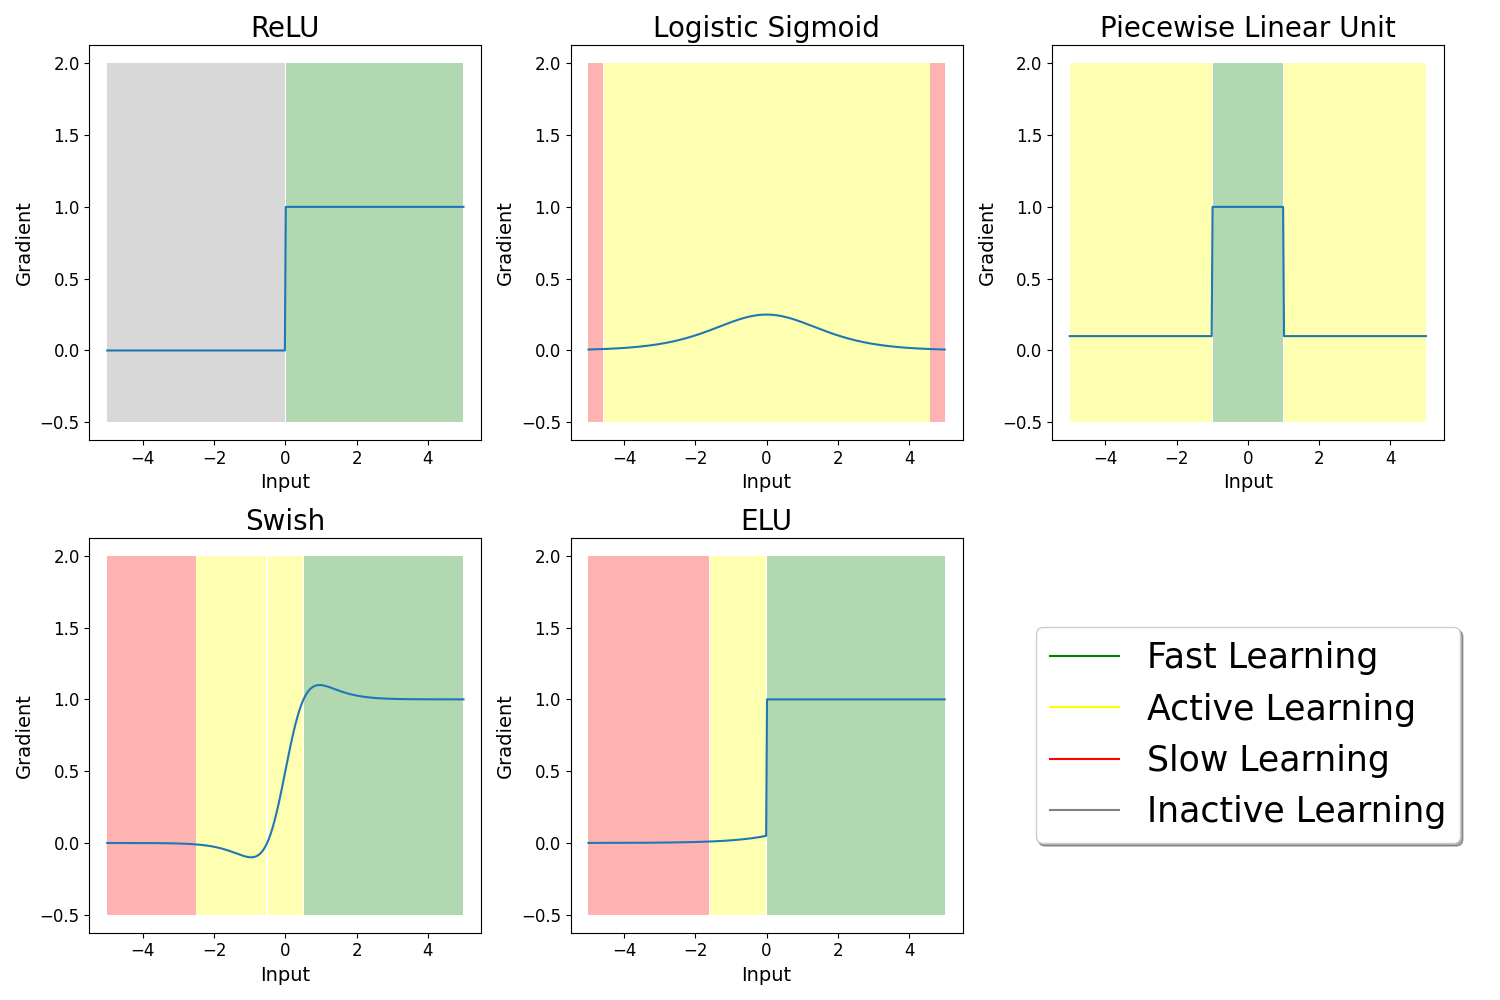
\includegraphics[width=18cm]{HW1/gradient_plot_q1.png}
    \caption{The plot of the gradient of each function.}
    \label{fig:gradients_q1}
\end{figure}

%----------------------------------------------------------------------------------------

\section*{Question 2}

\begin{problem}
Using a deep learning framework you have established, design and train a fully connected
ReLU neural network to approximate the following function:
\begin{equation}
    g(x) = \sin\left(\frac{\pi}{4}x\right)
\end{equation}
Here all the activation functions in the neural network are ReLU except the output layer, where the linear function
is used. Note that your neural network should have as few as possible neurons in the hidden layer(s) and the
largest error (i.e., the absolute difference between g(x) and the output of your neural network) should be no more
than 0.05 in the range of inputs from -2 to 2. You can generate and use no more than 200 training samples.
(a) Plot the training error with respect to the epoch along with the average and maximal error of the network
at the end of the epoch for the inputs from -2 to 2.
(b) Note that nonlinearity is essential for (deep) neural networks as one with no nonlinearity is reduced to a
one-layer neural network. The nonlinearity of every ReLU neural network can be characterized using
activation patterns, along with the activation regions. For any valid input, the activation pattern of a ReLU
network is a binary string for all its ReLU neurons, where 1 is assigned to such a neuron whose gradient is
1 and 0 is assigned to such a neuron whose gradient is 0. An activation region consists of all the inputs
with the same binary activation string. Compute the activation regions for your trained network and color
them for the inputs from -2 to 2. For each activation region, give its activation pattern.
(c) One way to characterize the dynamics of a neural network during training is to quantify the activation
pattern changes. At the beginning and end of each epoch, compute the activation patterns for all the
training examples and then compute the sum of the Hamming distance between the binary activationpatterns at the beginning and end of the epoch over all the training samples. Then plot the total Hamming
distance with respect to the training epoch. Is the overall trend consistent with your expectation? Provide a
justification.
\end{problem}

%------------------------------------------------

\subsection*{Answer}


\begin{enumerate}[label = (\alph*)]
	\item 
\end{enumerate}

%----------------------------------------------------------------------------------------

\section*{Question 3}

\begin{problem}
	Identify the author of Equation \ref{eq:bayes} below and briefly describe it in Latin.
	
	\medskip
	
	\begin{equation}\label{eq:bayes}
		P(A|B) = \frac{P(B|A)P(A)}{P(B)}
	\end{equation}
	
	\smallskip
\end{problem}

%------------------------------------------------

\subsection*{Answer} 

Lorem ipsum dolor sit amet, consectetur adipiscing elit. Praesent porttitor arcu luctus, imperdiet urna iaculis, mattis eros. Pellentesque iaculis odio vel nisl ullamcorper, nec faucibus ipsum molestie. Sed dictum nisl non aliquet porttitor. Etiam vulputate arcu dignissim, finibus sem et, viverra nisl. Aenean luctus congue massa, ut laoreet metus ornare in. Nunc fermentum nisi imperdiet lectus tincidunt vestibulum at ac elit. Nulla mattis nisl eu malesuada suscipit.

%----------------------------------------------------------------------------------------

\section*{Question 4 (bonus marks)}

\begin{problem}
	The table below shows the nutritional consistencies of two sausage types. Explain their relative differences given what you know about daily adult nutritional recommendations.
	
	\bigskip
    
	\begin{center}
		\begin{tabular}{l l l}
			\toprule
			\textit{Per 50g} & Pork & Soy \\
			\midrule
			Energy & 760kJ & 538kJ\\
			Protein & 7.0g & 9.3g\\
			Carbohydrate & 0.0g & 4.9g\\
			Fat & 16.8g & 9.1g\\
			Sodium & 0.4g & 0.4g\\
			Fibre & 0.0g & 1.4g\\
			\bottomrule
		\end{tabular}
	\end{center}
	
	\medskip
\end{problem}

%------------------------------------------------

\subsection*{Answer}

Lorem ipsum dolor sit amet, consectetur adipiscing elit. Praesent porttitor arcu luctus, imperdiet urna iaculis, mattis eros. Pellentesque iaculis odio vel nisl ullamcorper, nec faucibus ipsum molestie. Sed dictum nisl non aliquet porttitor. Etiam vulputate arcu dignissim, finibus sem et, viverra nisl. Aenean luctus congue massa, ut laoreet metus ornare in. Nunc fermentum nisi imperdiet lectus tincidunt vestibulum at ac elit. Nulla mattis nisl eu malesuada suscipit.

%----------------------------------------------------------------------------------------

\section*{Question 5 (bonus marks)}

\begin{problem}
	\lstinputlisting[
		caption=Luftballons Perl Script, % Caption above the listing
		label=lst:luftballons, % Label for referencing this listing
		language=Perl, % Use Perl functions/syntax highlighting
		frame=single, % Frame around the code listing
		showstringspaces=false, % Don't put marks in string spaces
		numbers=left, % Line numbers on left
		numberstyle=\tiny, % Line numbers styling
	]{}
	
	\begin{enumerate}
		\item How many luftballons will be output by the Listing \ref{lst:luftballons} above?
		\item Identify the regular expression in Listing \ref{lst:luftballons} and explain how it relates to the anti-war sentiments found in the rest of the script.
	\end{enumerate}

\end{problem}

%------------------------------------------------

\subsection*{Answer}

\begin{enumerate}
	\item 99 luftballons.
	\item Lorem ipsum dolor sit amet, consectetur adipiscing elit. Praesent porttitor arcu luctus, imperdiet urna iaculis, mattis eros. Pellentesque iaculis odio vel nisl ullamcorper, nec faucibus ipsum molestie. Sed dictum nisl non aliquet porttitor. Etiam vulputate arcu dignissim, finibus sem et, viverra nisl. Aenean luctus congue massa, ut laoreet metus ornare in. Nunc fermentum nisi imperdiet lectus tincidunt vestibulum at ac elit. Nulla mattis nisl eu malesuada suscipit.
\end{enumerate}

%----------------------------------------------------------------------------------------

\end{document}
